\section{Online synthesis}
Informally, the enforcer $S[u,t]$ onboard agent $u$ can only modify the trajectory of agent $u$. 
Every enforcer has access to a \emph{pathfinder} that modifies the corresponding trajectory. If a potential safety violation is detected, the enforcer on the agent with the lowest priority calls the pathfinder first. The order $\prec_t$ determines the next agent potentially required to modify its trajectory.
The pathfinder resolves conflicts, if any, within the group. If a new agent comes into the group, the pathfinder is called by the enforcer on the lowest priority agent. The trajectory of an agent is not modified if it is not involved in a safety violation. 
An \emph{ordering mechanism} maintains the order $\prec_t$ among the agents. When an agent reaches its final state, then its intended trajectory is updated and the ordering mechanism also updates the priorities.

\subsection{Pathfinder}

Informally, the pathfinder returns a new path whenever called. It constructs a graph and searches for a path in the graph from a vertex corresponding to the current location to a vertex in a target set corresponding to the agent's final state. This graph does not have any outgoing edges from vertices that correspond to unsafe configurations. After a single call to the pathfinder, the maximum length of the modified trajectory is at most $\ell + k$. where $\ell \leq k < d$ is some constant. But such a path may not always exist. In this case, the pathfinder returns a path that at the minimum keeps the system safe.

\paragraph*{Assumption}
The graph $G$ is 2-edge connected  and there is self loop on every vertex in $G$.

The self loop at every vertex in $G$ ensures that the agents can loiter.
%The alternate target set ensures safety and the that the agents is at most $k$ steps away from its final state. 
For any agent $u \in \Agents$, its trajectory $p_u$ is $p_u=(v_u,w_u)$.
%such that \Dj{$|w_u| \leq \ell \leq d$}, i.e., the next goal for any agent is some state that is visible to it. 
The final state of agent $u$ is $v_u^f$ and $priority(u,t)$ is its priority at time $t$. 

%Formally, 

\begin{eg}
Figure \ref{fig:eg5} depicts the graph $G_{blue}^0$ constructed by the pathfinder on the blue agent for the example in Figure~\ref{fig:eg4}a. The initial position is 
$v_{init} = ((4,2),0)$ and the target set $F = \{((1,2),4),((1,2),5)),((1,2),6))\}$ is marked red. The nodes occupied by some other higher priority agent at the time are marked by black circles. These black nodes do not have any out-edges. The pathfinder returns a path from $v_{init}$ to some vertex in $F$. The positions of the green agent are unmarked as it has a lower priority.
\begin{figure}[!htb]
    \centering
    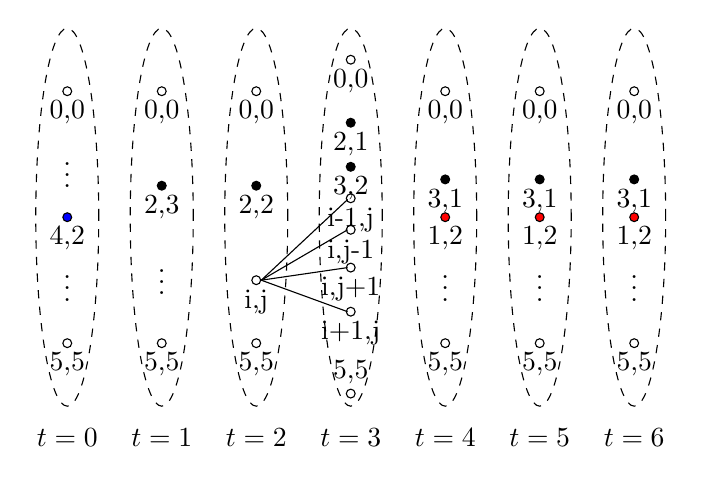
\begin{tikzpicture}[scale=0.8]
    \draw [dashed](0,0) ellipse (0.5cm and 3cm);
    \draw [dashed](1.5,0) ellipse (0.5cm and 3cm);
    \draw [dashed](3,0) ellipse (0.5cm and 3cm);
    \draw [dashed](4.5,0) ellipse (0.5cm and 3cm);
    \draw [dashed](6,0) ellipse (0.5cm and 3cm);
    \draw [dashed](7.5,0) ellipse (0.5cm and 3cm);
    \draw [dashed](9,0) ellipse (0.5cm and 3cm);
    \draw (0,-3.5) node {$t=0$};
    \draw (1.5,-3.5) node {$t=1$};
    \draw (3,-3.5) node {$t=2$};
    \draw (4.5,-3.5) node {$t=3$};
    \draw (6,-3.5) node {$t=4$};
    \draw (7.5,-3.5) node {$t=5$};
    \draw (9,-3.5) node {$t=6$};
    
    \draw (0,2) circle (2pt) node [anchor=north] {0,0};
    \draw (0,0.8) node {$\vdots$};
    \draw [fill = blue] (0,0) circle (2pt) node [anchor=north] {4,2};
    %\draw (0,-1.2) circle (1pt);
    \draw (0,-1) node {$\vdots$};
    %\draw (0,-0.8) circle (1pt);
    \draw (0,-2) circle (2pt) node [anchor=north] {5,5};
   
    \draw (1.5,2) circle (2pt) node [anchor=north] {0,0};
    \draw [fill = black] (1.5,0.5) circle (2pt) node [anchor=north] {2,3};
    %\draw [fill = black] (1.5,1) circle (2pt) node [anchor=north] {1,2};
    \draw (1.5,-2) circle (2pt) node [anchor=north] {5,5};
    
    \draw (1.5,-0.9) node {$\vdots$};
    %\draw (1.5,-1.2) circle (1pt);
    %\draw (1.5,-1) circle (1pt);
    %\draw (1.5,-0.8) circle (1pt);
    
    \draw (3,2) circle (2pt) node [anchor=north] {0,0};
    \draw [fill=black] (3,0.5) circle (2pt) node [anchor=north] {2,2};
    \draw (3,-2) circle (2pt) node [anchor=north] {5,5};
    \draw (3,-1) circle (2pt) node [anchor=north] {i,j};
   
    
    
    \draw (4.5,0.3) circle (2pt) node [anchor=north] {i-1,j};
    \draw (4.5,-0.2) circle (2pt) node [anchor=north] {i,j-1};
    \draw (4.5,-0.8) circle (2pt) node [anchor=north] {i,j+1};
    \draw (4.5,-1.5) circle (2pt) node [anchor=north] {i+1,j};
    
    \draw  (3.08,-1) -- (4.45,0.28);
    \draw  (3.08,-1) -- (4.45,-0.2);
    \draw  (3.08,-1) -- (4.45,-0.8);
    \draw  (3.08,-1) -- (4.45,-1.5);
    
    
    \draw (4.5,2.5) circle (2pt) node [anchor=north] {0,0};
    \draw [fill=black](4.5,0.8) circle(2pt) node[anchor = north] {3,2};
    \draw [fill=black](4.5,1.5) circle(2pt) node[anchor = north] {2,1};
    \draw (4.5,-2.8) circle (2pt) node [anchor=south] {5,5};
    
    \draw [fill=red] (6,0) circle (2pt)node [anchor=north] {1,2};
    \draw (6,2) circle (2pt) node [anchor=north] {0,0};
    \draw [fill=black](6,0.6) circle(2pt) node[anchor = north] {3,1};
    %\draw [fill=black](6,1.2) circle(2pt) node[anchor = north] {2,1};
    \draw (6,-2) circle (2pt) node [anchor=north] {5,5};
    
    %\draw (6,-1.2) circle (1pt);
    \draw (6,-1) node {$\vdots$};
    %\draw (6,-0.8) circle (1pt);
    
    
    \draw [fill=red] (7.5,0) circle (2pt)node [anchor=north] {1,2};
    \draw (7.5,2) circle (2pt) node [anchor=north] {0,0};
    \draw [fill=black](7.5,0.6) circle(2pt) node[anchor = north] {3,1};
    %\draw [fill=black](7.5,1.2) circle(2pt) node[anchor = north] {2,1};
    \draw (7.5,-2) circle (2pt) node [anchor=north] {5,5};
    
    %\draw (7.5,-1.2) circle (1pt);
    \draw (7.5,-1) node {$\vdots$};
    %\draw (7.5,-0.8) circle (1pt);
    
    
    \draw [fill=red] (9,0) circle (2pt)node [anchor=north] {1,2};
    \draw (9,2) circle (2pt) node [anchor=north] {0,0};
    \draw [fill=black](9,0.6) circle(2pt) node[anchor = north] {3,1};
    %\draw [fill=black](9,1.2) circle(2pt) node[anchor = north] {2,1};
    \draw (9,-2) circle (2pt) node [anchor=north] {5,5};
    %\draw (9,-1.2) circle (1pt);
    \draw (9,-1) node {$\vdots$};
    %\draw (9,-0.8) circle (1pt);
    
    \end{tikzpicture}
    \caption{The graph $G_{blue}^0$ (see Scenario~7) constructed by the pathfinder for the blue agent is shown. The set of vertices is $\{0,\dots5 \} \times \{0,\dots5 \} \times  \{ 0,\dots,6\}$. There is an edge between $((i,j),t_1)$ and $((i',j'),t_2)$ if and only if $|i'-i|+|j'-j| = 1$ and $t_2 = t_1 + 1$ and there is no out-edge from a black vertex (a black vertex corresponds to it being occupied by some agent at the corresponding time). $v_{init}$ is blue and the vertices in $F$ are red. The positions of the green agent are unmarked as it has a lower priority than the blue agent.}
    \label{fig:eg5}
\end{figure}
\end{eg}

%In \Dj{Example}~\ref{eg:collavoid}, we describe the graph and the initial and target states for the safety function corresponding to collision-avoidance \Dj{from} Example 3 for some agent \Dj{$u$.}
\begin{eg}\label{eg:collavoid}
For the safety function defined in Scenario~3, the 
pathfinder constructs the graph $G^t_{u} = (V', E')$ where $V'=V\times[t,t+d(v_u,v_u^f)+k]$. There is an edge with label $e$ between $(v,t)$ and $(v',t' +1)$, if in $G$ there is an edge $(v,v')$ with label $e$ and $\Vlabel(v,t') = \emptyset$, i.e., there are no higher priority agents occupying the same state. 
The target set $F$ is $\{(v^f_{u} ,t') | t+ d(v_u,v_u^f) \leq t' \leq t + d(v_u,v_u^f) + k\}$ and the initial state is $v_{init} = (v_{u},t)$. %\Dj{ The alternate target set 
%$F' = \{(v,t') | \Vlabel(v,t') = \emptyset~,t+ \ell \leq t' \leq t + \ell + k \}.$ 
%$F' = \{(v,k) | \Vlabel(v,k) = \emptyset~\text{and there is a path of length at most}~k~\text{between}~v~\text{and} ~v_u^f \}.$
%$F' = \{(v,t+1) | \Vlabel(v,t+1) = \emptyset \}.$
%The alternate target set corresponds to all the states that are not occupied by agents with higher priorities.
\end{eg}

\subsection{Occupancy graph}
The occupancy graph $O^t_u$ is similar to the pathfinder graph, however none of the edges are removed from the occupied states. The occupied states are labeled with the corresponding agents. Formally, the occupancy graph $O^t_{u} = (V', E')$ where $V'=V\times[t,t+d(v_u,v_u^f)+k] \setminus \{(v,t')|~v~$ is occupied by highest priority agent at $ t'\}$. There is an edge with label $e$ between $(v,t)$ and $(v',t' +1)$, if in $G$ there is an edge $(v,v')$ with label $e$. If $u' \in \Vlabel(v,t)$ and $priority(u) \geq priority(u')$, then $u' \in \Vlabel((v,t))$.  

\subsubsection{General pathfinder graph}

Next, we present the pathfinder construction for any local safety property $\Safety$ for agent $u$. For this, we need the safety function $\bar{\varphi}_u(t)$ defined as:
\begin{equation}
\label{eq:safety}
    \bar{\varphi}_u(t) \defeq \bigwedge_{priority(u)\leq priority(i)} \Safety_i(t).
\end{equation}
The safety function $\bar{\varphi}_u(t)$ ensures that all the agents with priorities higher than $u$ are safe.
$G_{u}^t = (V',E')$ is the graph whose nodes $V'$ are $V' = P \times [t,t+d(v_u,v_u^f)+k]$. Recall $P = V \times 2^\Agents$. There is an edge between $(v,t_1)$ to $(v',t_2)$ if i) $\Safety_u(v)  = \top$, ii) $(v,v')$ is an edge in $G$, iii) $t_2 = t_1 + 1$, iv) $\bar{\varphi}_u(t) = \top$, and v) all the other higher priority agents are following their trajectories, i.e., \begin{align}
        & u_i \in \Vlabel\left( \hat{\delta}(u_i^t,\prod_i W[0:t_1]),t_1 \right) \\
        \text{ and } 
        & u_i \in \Vlabel\left(( \hat{\delta}(u_i^t,\prod_i W[0:t_2]),t_2\right).
\end{align}
   
The initial vertex $v_{init}$ is $(a,t)$ where $a = v_u \times \Vlabel(v_u,t)$ and the set of target vertices $F$ is
$F=\{ (v,j)|v \in P' \text{ and } t+d(v_u,v_u^f) \leq j \leq t+d(v_u,v_u^f)+k \}$,
where $P' \subseteq P$ is a subset of all vertex labeling such that agent $u$ has reached its final state. %The alternate target set 
%$F' = \{ (v,t')~|~\bar{\Safety}_u(t') = \top \land u \in \Vlabel(v,t') \land t+ \ell \leq t' \leq t + \ell + k \}$.
%$F' = \{ (v,\ell)|\bar{\Safety}_u(\ell)=\top\land u\in\Vlabel(v,\ell)~\text{and there is a path of length at most}~\ell~\text{between}~v~\text{and} \\~v_u^f \}$.
%$F' = \{ (v,t+1)|\bar{\Safety}_u(t+1)=\top\land u\in\Vlabel(v,t+1)~\text{and there is a path of length at most}~\ell~\text{between}~v~\text{and} \\~v_u^f \}$.
Next, we describe the working of the pathfinder. The pathfinder constructs the graph $G_u^t$, initializes  $v_{init}$, a set $F$ of target vertices. The pathfinder then returns a path from $v_{init}$ to some state in $F$ if it exists, else it returns a random path of length 1 that only ensures safety. If no such path exists, the agent finds a shortest path in the occupancy graph to a vertex that ensures safety. This path may have other agents. All the other agents are forced to move 1 step along this path. If $p = v_1 v_2 \dots v_i v_{i+1}$ is the path from the occupancy graph, and agent $m$ is at $v_i$, then the trajectory of $m$ is replaced by $(v_i,v_{i+1})$. In short, if some lower priority agent cannot plan around the higher agent, then it might disturb all the agents other than the highest priority agent to ensure safety. However, the highest priority agent's path cannot be changed.
In the worst case, the pathfinder ensures that the agent with the highest priority can progress without any modifications. In essence lower priority agents progress, if they can plan around the highest priority agent.

\begin{algorithm}
\KwResult{Safe path for $u$}
Initialize $G_u^t$ and $O_u^t$\;
Initialize $v_{init}$ and $F$\;
$P$ = path in $G_u^t$ from $v_{init}$ to $F$\;
\If{$P$ exists}{return $p$\;}
\Else{
$P$ = shortest path to an unoccupied vertex in $O_u^t$\;
\ForAll{vertex $v_i \in P$}{
{
\If{$\Vlabel(v_i,t) = a$}{$w_a = (v_i,v_{i+1})$\;}
}
}

}
\caption{Pathfinder on agent $u$.}
\label{algo:pathfinder}
\end{algorithm}


%\Dj{For the collision avoidance safety property defined in Example \ref{eg:safety_fn} 
%\Dj{The assumption is \emph{not very} restrictive. If $G$ is connected and a centralized $\ell+k$--stabilizing shield can guarantee safety, then assumption 1 is satisfied.}
%minimum out degree of $G$ is greater than $\log_k |\Agents| / \log k$ and $\ell$ then assumption 1 is satisfied. The condition ensures that there at least one neighbor that is unoccupied. From a practical point of view, if the minimum degree is $4$ and $k = 10$ then we can handle collision avoidance for 1000 agents.




